% =====================================================================
%  Conference poster — A0 landscape
%  Single-Trajectory GRPO for Cooperative Multi-Agent RL  (Brian Ko, UW)
%  Build:  tectonic poster.tex
% =====================================================================
\documentclass[final]{beamer}
% 36 x 24 in landscape (91.44 x 60.96 cm) — required print size
\usepackage[size=custom,width=91.44,height=60.96,scale=0.88]{beamerposter}

\usepackage{lmodern}
\usepackage[T1]{fontenc}
\usepackage[scaled=0.95]{helvet}
\usepackage{amsmath,amssymb}
\usepackage{pifont}            % \ding checkmarks
\usepackage{qrcode}
\usepackage{tikz}
\usetikzlibrary{arrows.meta,positioning,calc}
\usepackage[most]{tcolorbox}

% ----------------------------- colors --------------------------------
\definecolor{uwpurple}{HTML}{4B2E83}   % UW Husky purple
\definecolor{uwpurpledk}{HTML}{36205F}
\definecolor{spiritgold}{HTML}{FFC700} % UW spirit gold
\definecolor{uwgold}{HTML}{B7A57A}     % UW metallic gold
\definecolor{pagebg}{HTML}{F5F4F8}
\definecolor{okblue}{HTML}{0072B2}     % Okabe–Ito, matches figure palette
\definecolor{okteal}{HTML}{009E73}     %   GRPO (step group-norm) curve
\definecolor{okverm}{HTML}{D55E00}     %   GRPO (global-norm) curve
\definecolor{okamber}{HTML}{E69F00}    %   MAPPO curve

\setbeamercolor{background canvas}{bg=pagebg}
\setbeamertemplate{navigation symbols}{}
\usefonttheme{professionalfonts}
\setbeamercolor{itemize item}{fg=uwpurple}
\setbeamercolor{itemize subitem}{fg=uwpurple}
\setbeamertemplate{itemize item}{\textcolor{spiritgold!70!black}{\raisebox{1pt}{\small$\blacktriangleright$}}}
\setbeamertemplate{itemize subitem}{\textcolor{uwpurple!60}{\raisebox{1pt}{\footnotesize$\triangleright$}}}
\setlength{\leftmargini}{1.6em}
\setlength{\leftmarginii}{1.4em}

\newcommand{\cmark}{\textcolor{okteal}{\ding{51}}}
\newcommand{\xmark}{\textcolor{okverm}{\ding{55}}}
\newcommand{\dsep}{\;\raisebox{0.45ex}{$\scriptstyle\bullet$}\;}

% ----------------------------- blocks --------------------------------
\newcommand{\numchip}[1]{%
  \tikz[baseline=-0.65ex]\node[circle,fill=spiritgold,text=uwpurpledk,
        inner sep=4pt,minimum size=1.05cm,font=\large\bfseries]{#1};}

\newtcolorbox{pblock}[2][]{%
  enhanced, colback=white, colframe=uwpurple!55, boxrule=1.1pt, arc=9pt,
  left=10pt, right=10pt, top=5pt, bottom=7pt,
  toptitle=4pt, bottomtitle=4pt, titlerule=0pt,
  colbacktitle=uwpurple, coltitle=white, fonttitle=\Large\bfseries,
  title={#2}, #1}

\newtcolorbox{statbox}[1][]{%
  colback=uwpurple!7, colframe=uwpurple!35, boxrule=0.8pt, arc=7pt,
  left=6pt, right=6pt, top=7pt, bottom=7pt, halign=center, #1}

\newcommand{\blockgap}{\par\vspace{0.3cm}}
\newcommand{\figcap}[1]{{\centering\small\bfseries\color{uwpurple} #1\par}}

% =====================================================================
\begin{document}
\begin{frame}[t]
\vspace*{-0.15cm}

% ============================ HEADER =================================
\begin{tcolorbox}[enhanced, colback=uwpurple, colframe=uwpurple, arc=12pt,
                  left=17pt, right=17pt, top=10pt, bottom=10pt]
\begin{minipage}[c]{0.835\linewidth}
  {\large\bfseries\color{spiritgold}
    UNIVERSITY OF WASHINGTON \quad\textcolor{white!70!uwpurple}{$\vert$}\quad
    PREPRINT --- UNDER REVIEW}\\[0.33cm]
  {\fontsize{58}{64}\selectfont\bfseries\color{white}
    Single-Trajectory GRPO for Cooperative\\[0.07cm]
    Multi-Agent Reinforcement Learning\par}
  \vspace{0.33cm}
  {\LARGE\color{white} Brian Ko}\quad
  {\Large\color{white!75!uwpurple} University of Washington \dsep
   \texttt{kkm97183@uw.edu}}
\end{minipage}\hfill
\begin{minipage}[c]{0.135\linewidth}
  \begin{tcolorbox}[colback=white, colframe=white, arc=7pt, halign=center,
                    left=4pt,right=4pt,top=7pt,bottom=7pt]
    \qrcode[height=4.1cm]{https://github.com/ko120/IGRPO}\\[0.25cm]
    {\normalsize\bfseries\color{uwpurpledk} Paper + code}\\
    {\small\color{black!60}\texttt{github.com/ko120/IGRPO}}
  \end{tcolorbox}
\end{minipage}
\end{tcolorbox}

\vspace{0.25cm}

% ============================ TL;DR strip ============================
\begin{tcolorbox}[colback=spiritgold!88!white, colframe=spiritgold!88!white,
                  arc=9pt, left=13pt, right=13pt, top=7pt, bottom=7pt]
  \centering {\LARGE\bfseries\color{uwpurpledk}
  TL;DR \;---\; The $n$ agents inside one episode form the GRPO group:
  critic-free MARL matches PPO with $\mathbf{16\%}$ less peak GPU memory ---
  normalize returns globally over agents and time, not per time step.}
\end{tcolorbox}

\vspace{0.42cm}

% ============================ BODY ===================================
\noindent
% ----------------------------------------------------------- COLUMN 1
\begin{minipage}[t]{0.312\textwidth}\vspace{0pt}

\begin{pblock}{\numchip{1}\; Why critic-free MARL?}
\begin{itemize}\setlength\itemsep{0.16cm}
  \item PPO-style MARL (IPPO, MAPPO) trains a \textbf{critic + GAE}:
        extra memory, extra compute, and value-estimation error.
  \item \textbf{GRPO} drops the critic: advantages are rewards normalized
        across a \emph{group of rollouts of the same prompt} --- the recipe
        behind LLM post-training (DeepSeekMath).
  \item In MARL we do \textbf{not} get many rollouts from an identical state
        --- so where does the group come from?
  \item \textbf{Our answer:} in homogeneous cooperative MARL, the $n$ agents
        inside \emph{one} episode already form the group.
\end{itemize}
\end{pblock}

\blockgap

\begin{pblock}{\numchip{2}\; Key idea: the agents are the group}
\centering
\resizebox{0.9\linewidth}{!}{%
\begin{tikzpicture}[
  font=\small,
  bx/.style={rounded corners=5pt, draw=black!35, fill=black!5,
             inner sep=7pt, align=center},
  gd/.style={rounded corners=6pt, draw=uwgold!90!black, line width=1.2pt,
             fill=spiritgold!22, inner sep=9pt, align=center},
  arr/.style={-{Stealth[length=9pt]}, line width=1.6pt, draw=black!50}]
  % ---------- top panel: LLM GRPO ----------
  \node[anchor=west, font=\small\bfseries, text=black!55] at (0,11.1)
        {Standard GRPO (LLM post-training)};
  \node[bx] (prompt) at (1.7,9.3) {prompt $x$};
  \node[bx, minimum width=3.4cm] (c1) at (7.0,10.35) {$y_1 \;\to\; r_1$};
  \node[bx, minimum width=3.4cm] (c2) at (7.0, 9.30) {$y_2 \;\to\; r_2$};
  \node[bx, minimum width=3.4cm] (c3) at (7.0, 8.25) {$y_G \;\to\; r_G$};
  \node[gd] (g1) at (14.6,9.3)
        {group $=$ $G$ rollouts of the\\ \emph{same} prompt:\;
         $\hat A_k=\frac{r_k-\mu}{\sigma}$};
  \draw[arr] (prompt) -- (c1.west);
  \draw[arr] (prompt) -- (c2.west);
  \draw[arr] (prompt) -- (c3.west);
  \draw[arr] (c1.east) -- (g1.west|-c1.east);
  \draw[arr] (c2.east) -- (g1.west);
  \draw[arr] (c3.east) -- (g1.west|-c3.east);
  \node[anchor=west, font=\small\bfseries, text=okverm] at (0,7.3)
        {\xmark\; needs many rollouts from the same state --- unavailable in MARL};
  \draw[dash pattern=on 6pt off 5pt, black!25, line width=1pt]
        (0,6.55) -- (18.4,6.55);
  % ---------- bottom panel: ours ----------
  \node[anchor=west, font=\small\bfseries, text=uwpurple] at (0,5.85)
        {This work: single-trajectory GRPO};
  \draw[rounded corners=8pt, draw=uwpurple!60, line width=1.4pt, fill=white]
        (0.0,0.55) rectangle (10.6,5.25);
  \node[anchor=north west, font=\footnotesize\bfseries, text=uwpurple!80]
        at (0.15,5.2) {one episode};
  \foreach \i/\yy/\cc in {1/4.05/okblue, 2/2.85/okamber, 3/1.65/okteal}{
    \node[anchor=east, font=\footnotesize, text=black!65] at (1.95,\yy)
          {agent $\i$};
    \foreach \k in {0,...,6}
      \fill[\cc!80] ($(2.25+\k*0.92,\yy)$) ++(-0.30,-0.30)
            rectangle ++(0.60,0.60);
    \node[anchor=west, font=\small] at (8.6,\yy) {$\to\,G_{\i,t}$};
  }
  \node[gd] (g2) at (14.6,2.9)
        {group $=$ $n$ agents $\times$ $T$ steps\\[2pt]
         $\hat A_{i,t}=\dfrac{G_{i,t}-\mu}{\sigma}$};
  \draw[arr] (10.6,2.9) -- (g2.west);
  \node[rounded corners=14pt, fill=uwpurple, text=white,
        font=\small\bfseries, inner sep=9pt] at (14.6,0.85)
        {no critic \dsep no GAE \dsep no extra rollouts};
\end{tikzpicture}}
\end{pblock}

\blockgap

\begin{pblock}{\numchip{3}\; Method}
\textbf{PPO-like clipped objective, KL-regularized, critic-free:}
\vspace{-0.15cm}
\begin{equation*}
  J(\theta)=\mathbb{E}\!\left[\min\!\big(r\,\hat A,\;
  \operatorname{clip}(r,1\!-\!\epsilon,1\!+\!\epsilon)\,\hat A\big)\right]
  -\beta\,\mathrm{KL}\!\left(\pi_\theta\,\Vert\,\pi_{\text{ref}}\right)
\end{equation*}
value-loss coefficient $0$, no entropy bonus, value targets $\equiv 0$.
Advantages built from \textbf{discounted returns-to-go}
$\;G_{i,t}=\sum_{\tau} \gamma^{\tau} R(s_{i,t+\tau},u_{i,t+\tau})$.

\vspace{0.25cm}
\begin{tcolorbox}[colback=okteal!6, colframe=okteal!70, boxrule=1.2pt,
                  arc=6pt, left=7pt, right=7pt, top=6pt, bottom=6pt]
  \textbf{\textcolor{okteal!60!black}{A) Per-time-step cross-agent}}
  \hfill {\small (Zhao \& Li, 2025)}\\[2pt]
  $\hat A_{i,t}=\frac{G_{i,t}-\mu_t}{\sigma_t}$, \;
  $(\mu_t,\sigma_t)$ over the $n$ agents at step $t$
  \;$\Rightarrow$\; only $n{=}3$ samples per step, and advantages are
  \textbf{zero-sum across agents at every step}.
\end{tcolorbox}
\vspace{0.18cm}
\begin{tcolorbox}[colback=okverm!6, colframe=okverm!75, boxrule=1.2pt,
                  arc=6pt, left=7pt, right=7pt, top=6pt, bottom=6pt]
  \textbf{\textcolor{okverm!75!black}{B) Global episode statistics}}
  \hfill {\small (this work)}\\[2pt]
  $\hat A_{i,t}=\frac{G_{i,t}-\mu}{\sigma}$, \;
  one $(\mu,\sigma)$ over \emph{all} $n\,T$ values $\{G_{i,t}\}$
  \;$\Rightarrow$\; $n\,T$-sample baseline that \textbf{preserves absolute
  return differences} within the episode.
\end{tcolorbox}
\vspace{0.22cm}
\textbf{Drop-in:} swaps RLlib's GAE connector for a group-normalization
connector --- everything else is standard PPO machinery.
\end{pblock}

\end{minipage}\hfill
% ----------------------------------------------------------- COLUMN 2
\begin{minipage}[t]{0.348\textwidth}\vspace{0pt}

\begin{pblock}{\numchip{4}\; Setup: two sparse-reward gridworlds}
\begin{minipage}[t]{0.485\linewidth}
  \textbf{\textcolor{uwpurple}{Cluttered $15{\times}15$}}\\
  30 fixed obstacles, fixed goal, randomized starts --- moderate difficulty.
\end{minipage}\hfill
\begin{minipage}[t]{0.485\linewidth}
  \textbf{\textcolor{uwpurple}{FourRooms $15{\times}15$}}\\
  doorways, goal, \emph{and} starts all randomized each reset --- hard
  exploration.
\end{minipage}
\vspace{0.22cm}

{\small $n{=}3$ agents \dsep egocentric $5{\times}5{\times}3$ obs \dsep
7 actions \dsep $\le 100$ steps \dsep parameter sharing (CTDE)
\dsep reward only on reaching the goal:
$\;r = 1-\frac{\texttt{step\_count}}{\texttt{max\_steps}}$, else $0$
\dsep 3 seeds, mean $\pm$ SEM \dsep built on RLlib.\par}
\end{pblock}

\blockgap

\begin{pblock}{\numchip{5}\; Main result --- GRPO matches PPO with less memory
               \;{\normalsize(RQ3)}}
\begin{minipage}[t]{0.46\linewidth}
  \figcap{Cluttered}
  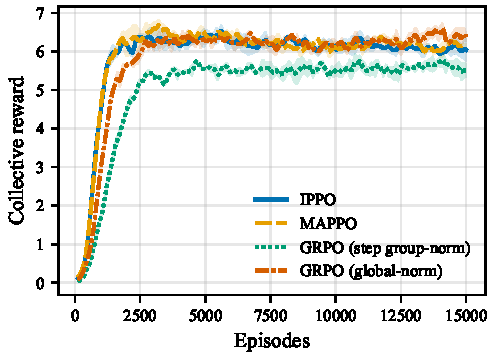
\includegraphics[width=\linewidth]{figures/cluttered_reward.pdf}
\end{minipage}\hfill
\begin{minipage}[t]{0.46\linewidth}
  \figcap{FourRooms}
  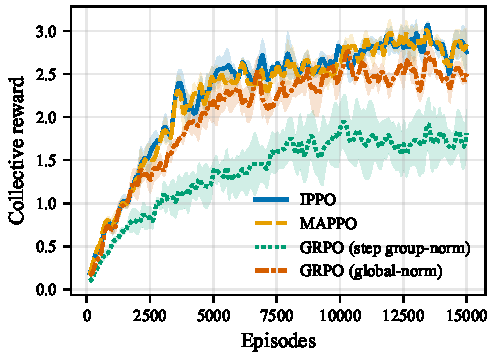
\includegraphics[width=\linewidth]{figures/fourrooms_reward.pdf}
\end{minipage}

\vspace{0.2cm}
\begin{minipage}[c]{0.43\linewidth}
  \figcap{Peak GPU memory per run}
  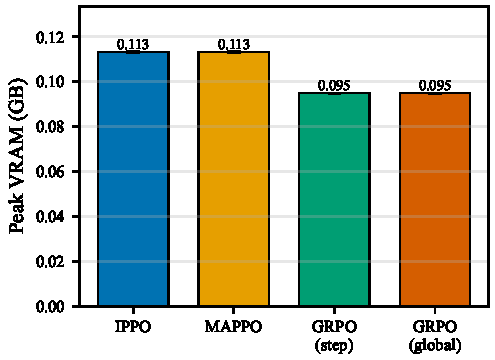
\includegraphics[width=\linewidth]{figures/fig1_vram.pdf}
\end{minipage}\hfill
\begin{minipage}[c]{0.54\linewidth}
  \begin{statbox}
    {\fontsize{42}{44}\selectfont\bfseries\color{uwpurple} $-16\%$}\\[3pt]
    {\large\bfseries peak VRAM, critic-free}\\[2pt]
    {\small\color{black!60} $0.113$\,GB $\to$ $0.095$\,GB}
  \end{statbox}
  \vspace{0.16cm}
  \begin{statbox}
    {\Large\bfseries\color{uwpurple} $6.4\pm0.2$ \;vs.\; $6.1\pm0.1$}\\[2pt]
    {\small\color{black!60} GRPO (global) vs.\ IPPO --- Cluttered}
  \end{statbox}
  \vspace{0.16cm}
  \begin{statbox}
    {\Large\bfseries\color{uwpurple} $2.5\pm0.1$ \;vs.\; $2.8\pm0.1$}\\[2pt]
    {\small\color{black!60} GRPO (global) vs.\ IPPO --- FourRooms}
  \end{statbox}
\end{minipage}

\vspace{0.2cm}
\textbf{Takeaway:} \textcolor{okverm}{GRPO (global-norm)} reaches IPPO-level
reward on both environments with \textbf{no critic} --- comparable
wall-clock, $16\%$ lower peak VRAM at this model scale.
\end{pblock}

\blockgap

\begin{pblock}{\numchip{6}\; PPO design choices \;{\normalsize(RQ1--RQ2)}}
\begin{minipage}[c]{0.31\linewidth}
  \figcap{Runtime, 30k episodes}
  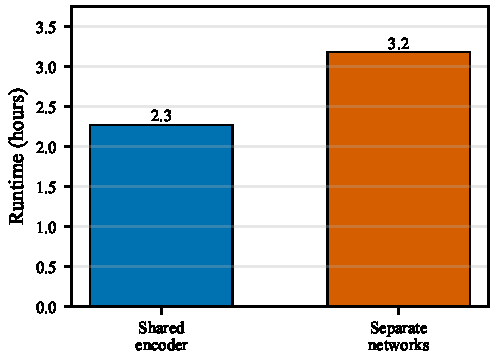
\includegraphics[width=\linewidth]{figures/fig2_runtime.pdf}
\end{minipage}\hfill
\begin{minipage}[c]{0.66\linewidth}
\begin{itemize}\setlength\itemsep{0.16cm}
  \item \textbf{Shared encoder $\approx$ separate networks} in sample
        efficiency, but $\mathbf{30\%}$ \textbf{less wall-clock}
        ($2.3$ vs.\ $3.2$\,h).
  \item \textbf{MAPPO $=$ IPPO under sparse rewards}: the centralized
        critic adds no measurable benefit ($6.1\pm0.1$ / $2.8\pm0.1$ for
        both). More information $\neq$ better.
\end{itemize}
\end{minipage}
\end{pblock}

\end{minipage}\hfill
% ----------------------------------------------------------- COLUMN 3
\begin{minipage}[t]{0.312\textwidth}\vspace{0pt}

\begin{pblock}{\numchip{7}\; The group statistics are the critical choice
               \;{\normalsize(RQ4)}}
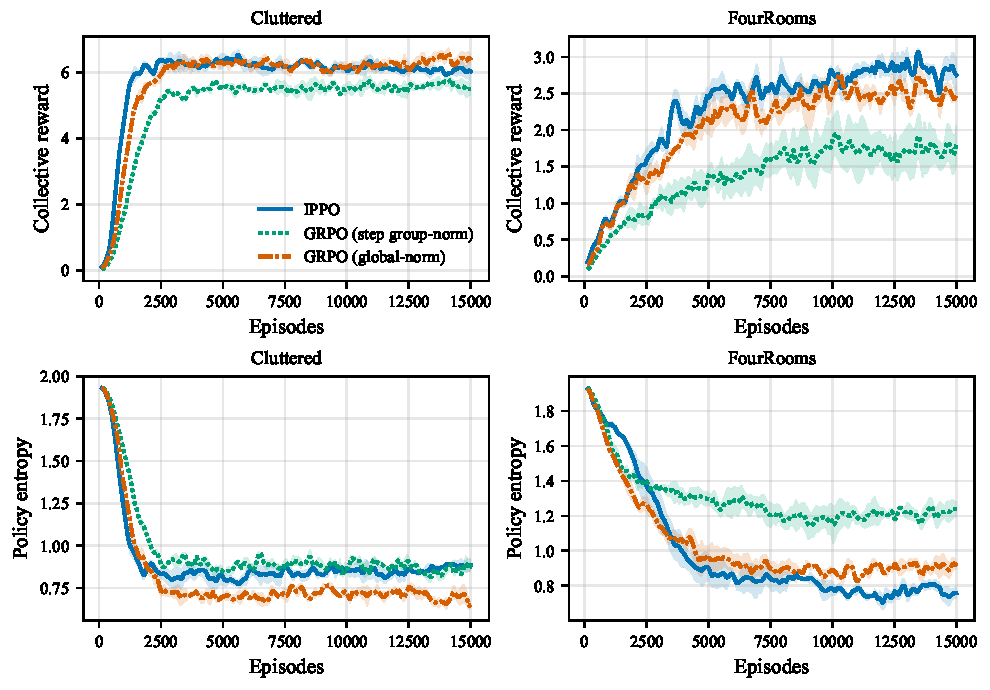
\includegraphics[width=\linewidth]{figures/fig4_norm.pdf}
{\small\color{black!60} Top: collective reward. Bottom: policy entropy.
 Cluttered (left), FourRooms (right).}
\vspace{0.18cm}
\begin{itemize}\setlength\itemsep{0.16cm}
  \item On Cluttered both variants learn; on FourRooms
        \textcolor{okteal}{\textbf{per-time-step}} \textbf{collapses}:
        plateaus at $1.7\pm0.3$ (vs.\ IPPO $2.8\pm0.1$) with entropy stuck
        high --- \textcolor{okverm}{\textbf{global}} stays competitive
        ($2.5\pm0.1$).
  \item \textbf{Why:} $(\mu_t,\sigma_t)$ are estimated from only $n{=}3$
        returns per step; under sparse reward the three returns are often
        identical (all zero) $\Rightarrow$ advantage collapses to zero ---
        no learning signal.
  \item \textbf{Zero-sum grading:} even when \emph{all} agents succeed,
        slower agents get negative advantage.
  \item Global pools $n\,T$ samples into one stable baseline; with
        lateness-scaled rewards bounded in $[0,1]$, return scales stay
        comparable across time, so one global mean is a sound baseline.
\end{itemize}
\end{pblock}

\blockgap

\begin{tcolorbox}[enhanced, colback=uwpurple, colframe=uwpurple, arc=9pt,
                  left=12pt, right=12pt, top=10pt, bottom=10pt]
{\Large\bfseries\color{spiritgold} Takeaways}\\[0.25cm]
{\color{white}
\cmark\; \textbf{Critic-free GRPO is a practical CTDE recipe}: matches
IPPO/MAPPO on both tasks with $16\%$ less peak VRAM.\\[0.22cm]
\cmark\; \textbf{Normalize globally} over agents $\times$ timesteps ---
per-time-step cross-agent statistics fail on hard exploration.\\[0.22cm]
\cmark\; \textbf{Centralization is not free lunch}: MAPPO's global critic
adds nothing under sparse rewards; shared encoders cut runtime $30\%$.
\\[0.33cm]
{\small\color{white!75!uwpurple}\textbf{Limitations:} two gridworlds from one
family, $n{=}3$, small CNNs (absolute VRAM saving modest); formal variance
analysis of single-trajectory baselines left to future work.}}
\end{tcolorbox}

\end{minipage}

% ============================ FOOTER =================================
\vspace{0.1cm}
\begin{center}
{\small\color{black!55}
\textbf{References:} Schulman et al., PPO, 2017 \dsep
Yu et al., MAPPO/IPPO, NeurIPS 2022 \dsep
Shao et al., DeepSeekMath (GRPO), 2024 \dsep
Zhao \& Li, one-step MARL GRPO, 2025 \dsep
Liang et al., RLlib, 2018
\qquad\textcolor{black!30}{$\vert$}\qquad
code \& configs: \texttt{github.com/ko120/IGRPO}}
\end{center}

\end{frame}
\end{document}
